\chapter{Networks implementation}
In this chapter, detailed description of each implemented network is presented. All topologies were designed to be as similar as possible, with the only exception for details characteristic for given method. Such approach ensures that all differences in results arise from the exceptional quality of particular technique. In case of methods incorporating autoencoders approach, size of encoded latent face was set to 200.\\

Types of layers used in models implementations are: fully connected layer, 2D convolution layer, transposed 2D convolution layer, flatten layer and lambda layer (to apply desired function when constructing customized layer). Activation functions applied to different layers are presented in figure \ref{fig:activation_functions}. Additionally, to improve stability of the training process, batch normalization and instance normalization were applied to selected layers.

\begin{figure}[H]
\centering
\begin{subfigure}{.32\textwidth}
  \centering
  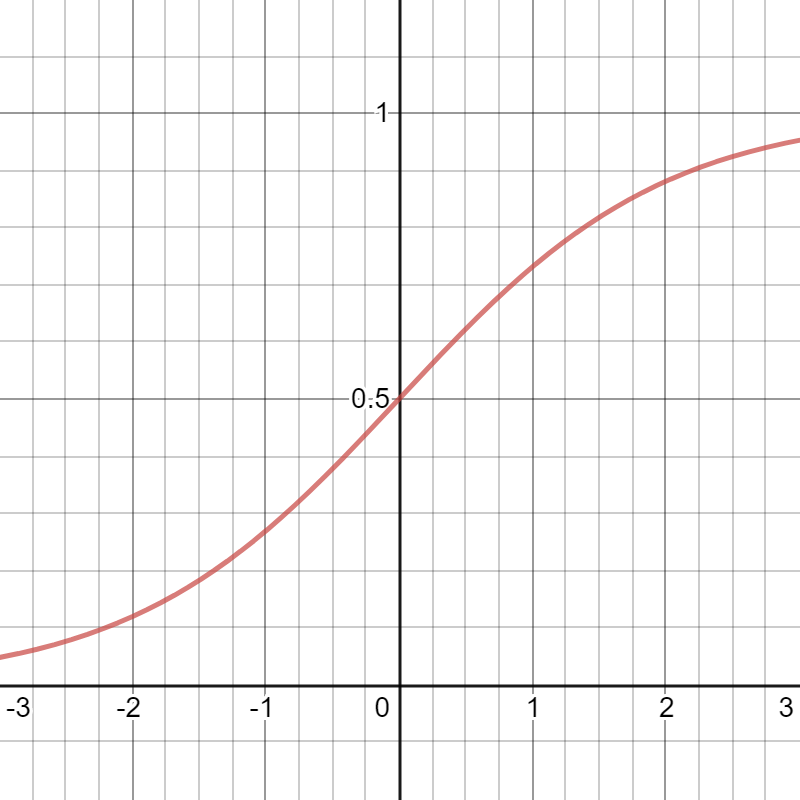
\includegraphics[width=0.9\linewidth]{activation_function_1.png}
  \caption{Sigmoid}
  \label{subfig:activation_function_1}
\end{subfigure}%
\begin{subfigure}{.32\textwidth}
  \centering
  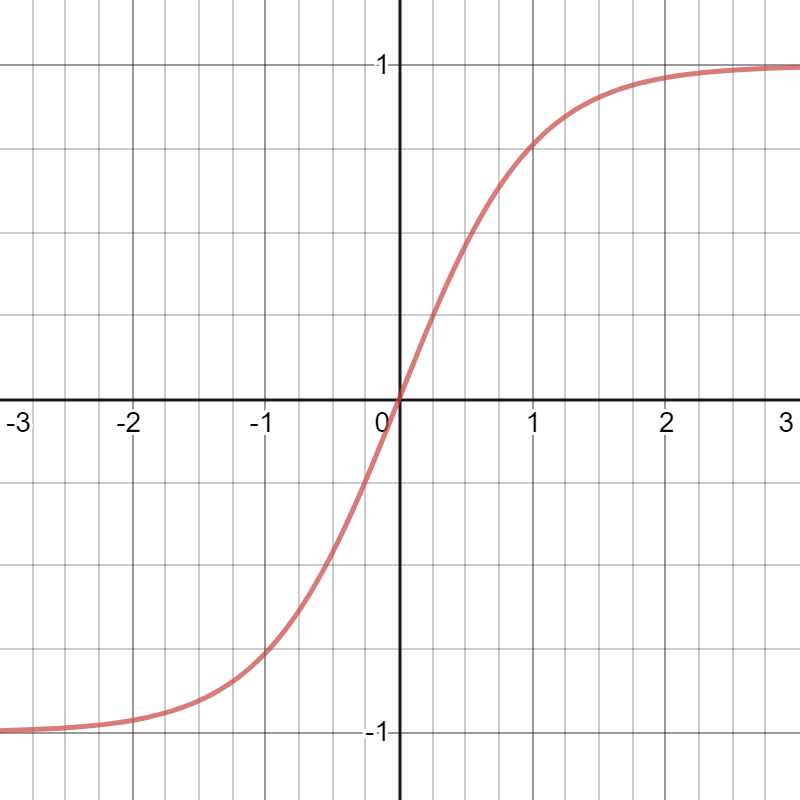
\includegraphics[width=0.9\linewidth]{activation_function_2.png}
  \caption{Tanh}
  \label{subfig:activation_function_2}
\end{subfigure}
\vskip\baselineskip
\begin{subfigure}{.32\textwidth}
  \centering
  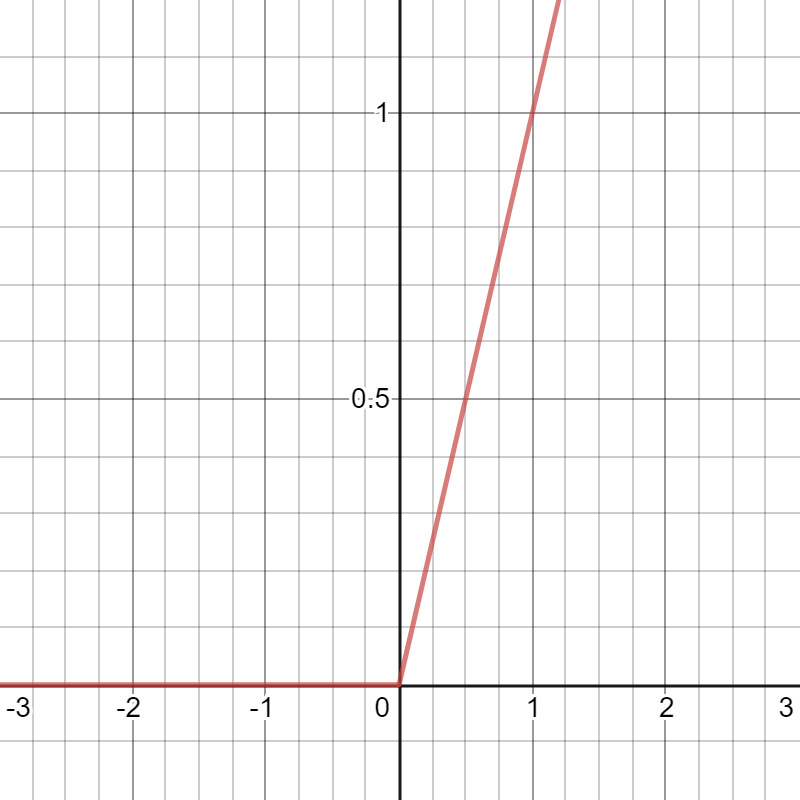
\includegraphics[width=0.9\linewidth]{activation_function_3.png}
  \caption{ReLU}
  \label{subfig:activation_function_3}
\end{subfigure}%
\begin{subfigure}{.32\textwidth}
  \centering
  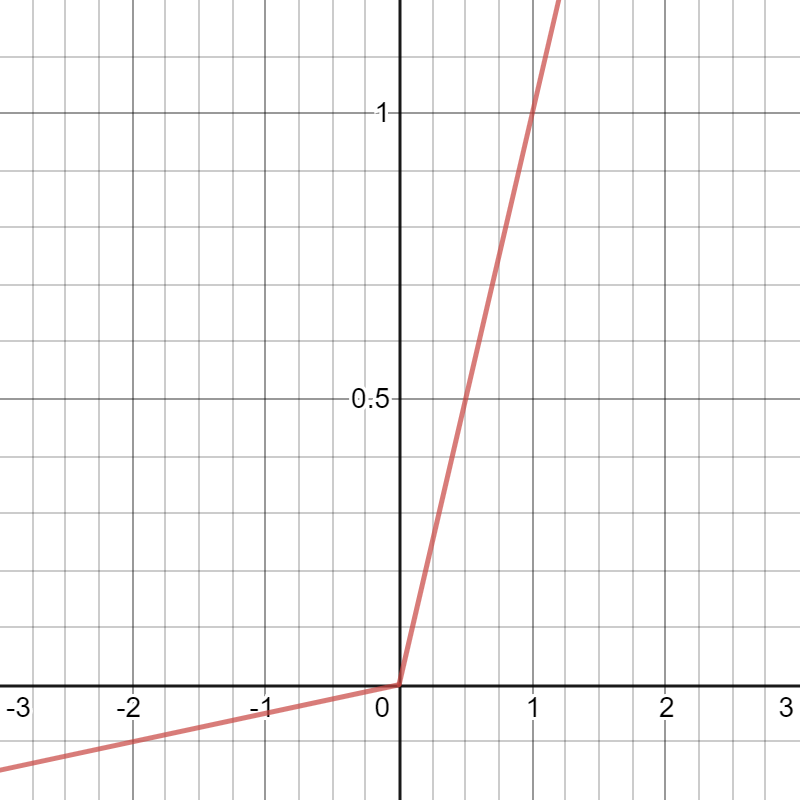
\includegraphics[width=0.9\linewidth]{activation_function_4.png}
  \caption{LeakyReLU}
  \label{subfig:activation_function_4}
\end{subfigure}
\caption{Applied activation functions}
\label{fig:activation_functions}
\end{figure}

\section{Autoencoder}

\begin{figure}[H]
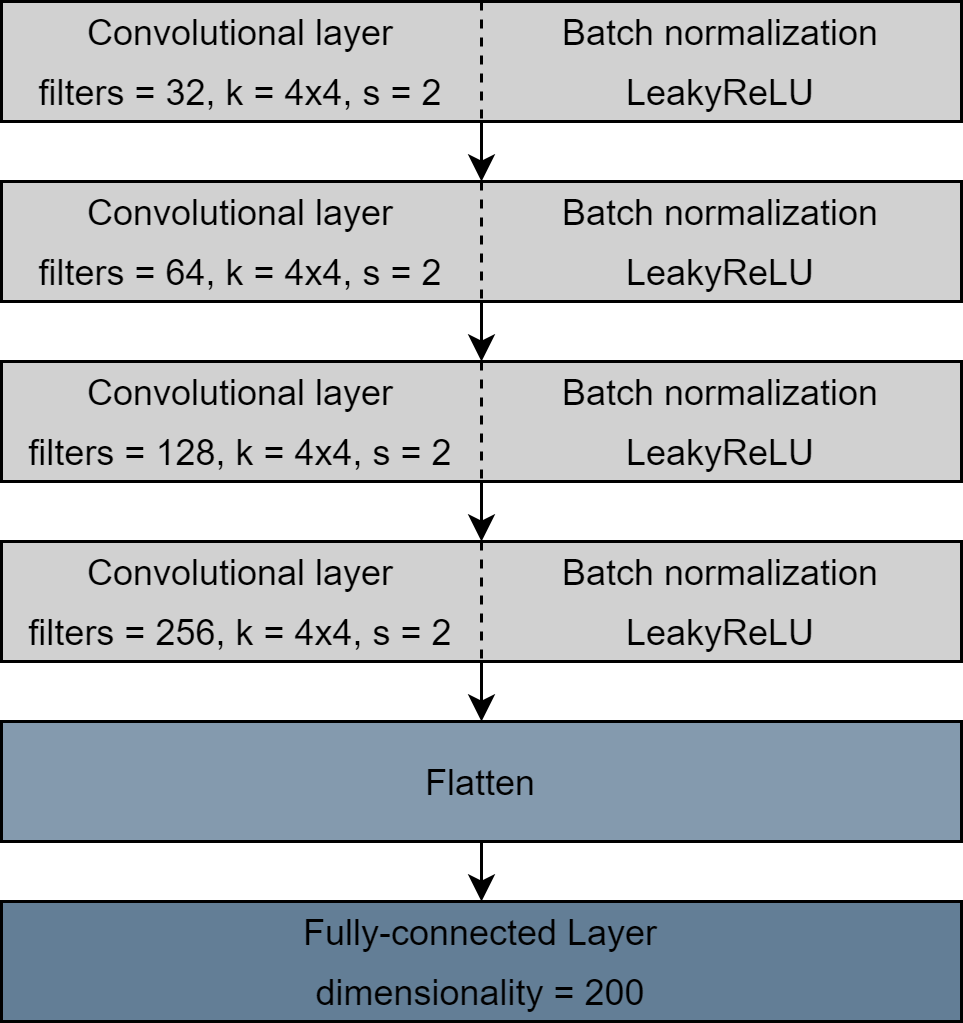
\includegraphics[width=10cm] {Models/ae_encoder.png}
\centering
\caption{Encoder architecture}
\label{fig:ae_encoder}
\end{figure}

\begin{figure}[H]
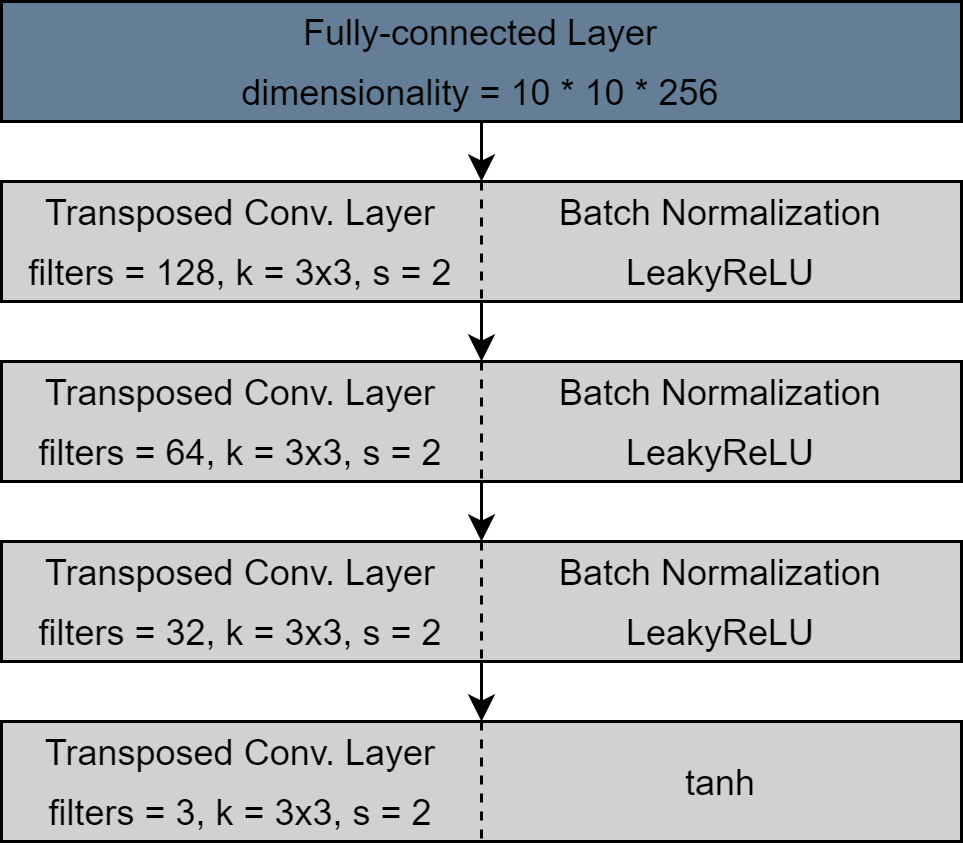
\includegraphics[width=10cm] {Models/ae_decoder.png}
\centering
\caption{Decoder architecture}
\label{fig:ae_decoder}
\end{figure}

\section{Variational autoencoder}

\begin{figure}[H]
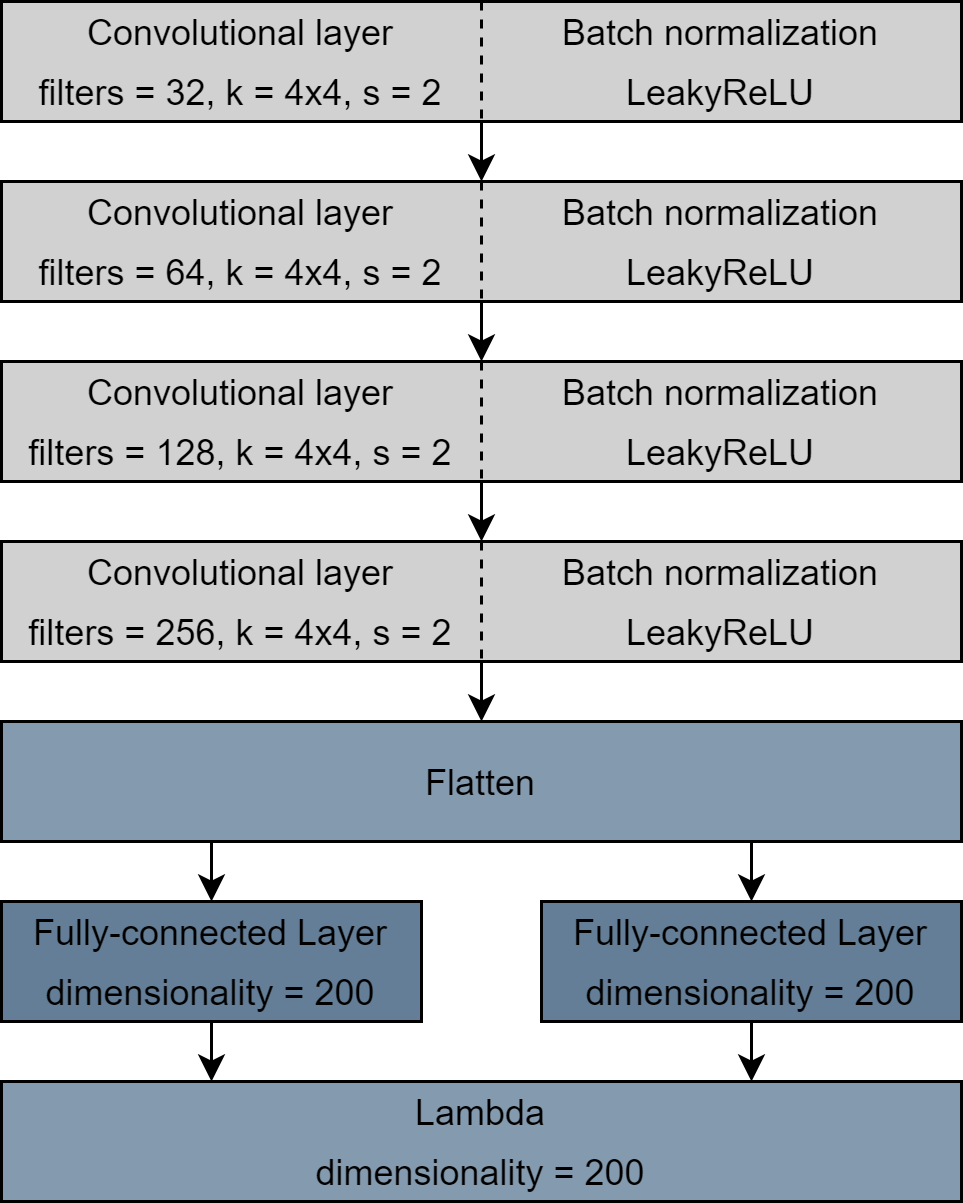
\includegraphics[width=10cm] {Models/vae_encoder.png}
\centering
\caption{Encoder architecture}
\label{fig:vae_encoder}
\end{figure}

\begin{figure}[H]
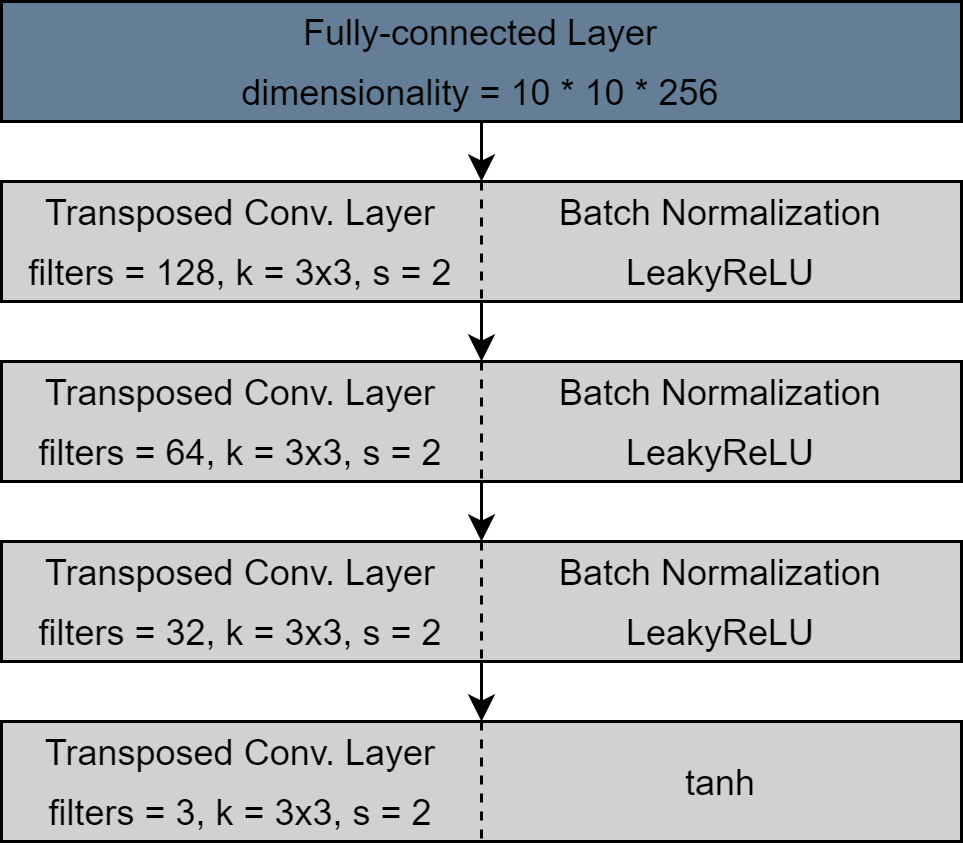
\includegraphics[width=10cm] {Models/vae_decoder.png}
\centering
\caption{Decoder architecture}
\label{fig:vae_decoder}
\end{figure}

\section{VAE-GAN}

\begin{figure}[H]
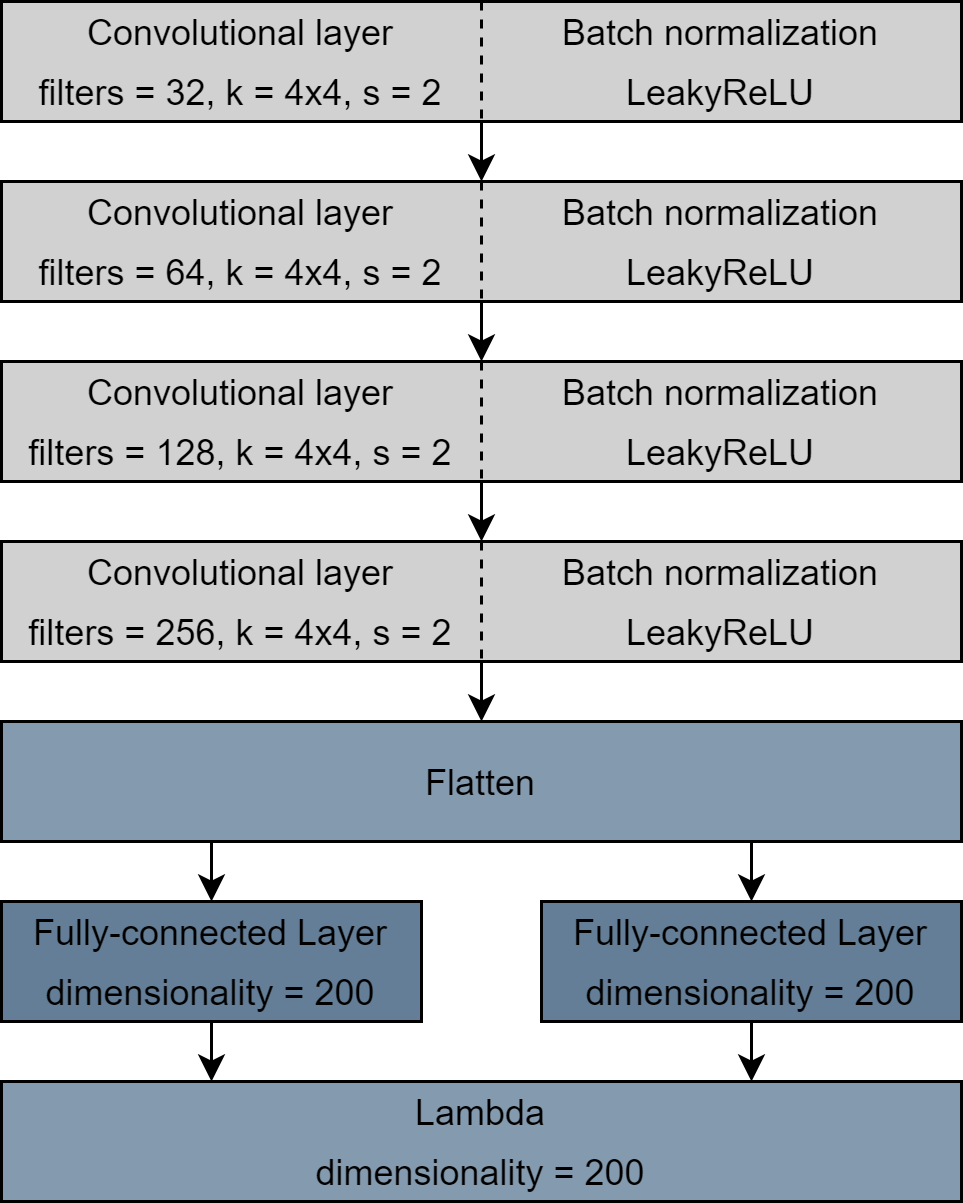
\includegraphics[width=10cm] {Models/vaegan_encoder.png}
\centering
\caption{Encoder architecture}
\label{fig:vaegan_encoder}
\end{figure}

\begin{figure}[H]
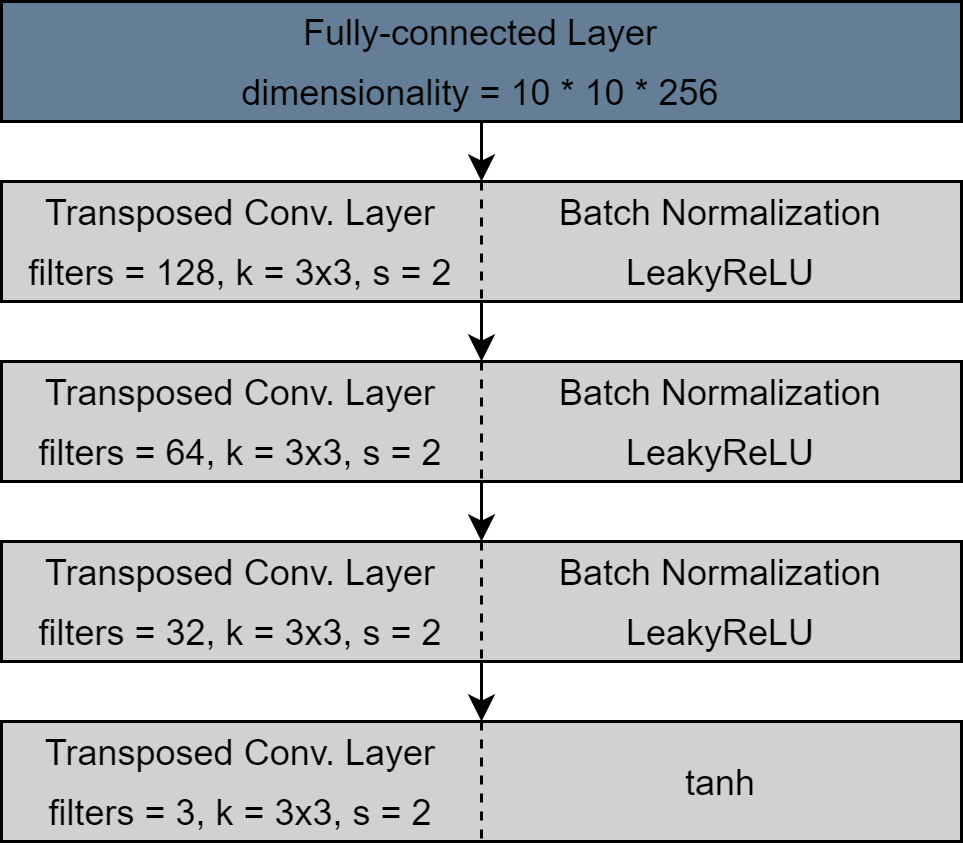
\includegraphics[width=10cm] {Models/vaegan_generator.png}
\centering
\caption{Generator architecture}
\label{fig:vaegan_generator}
\end{figure}

\begin{figure}[H]
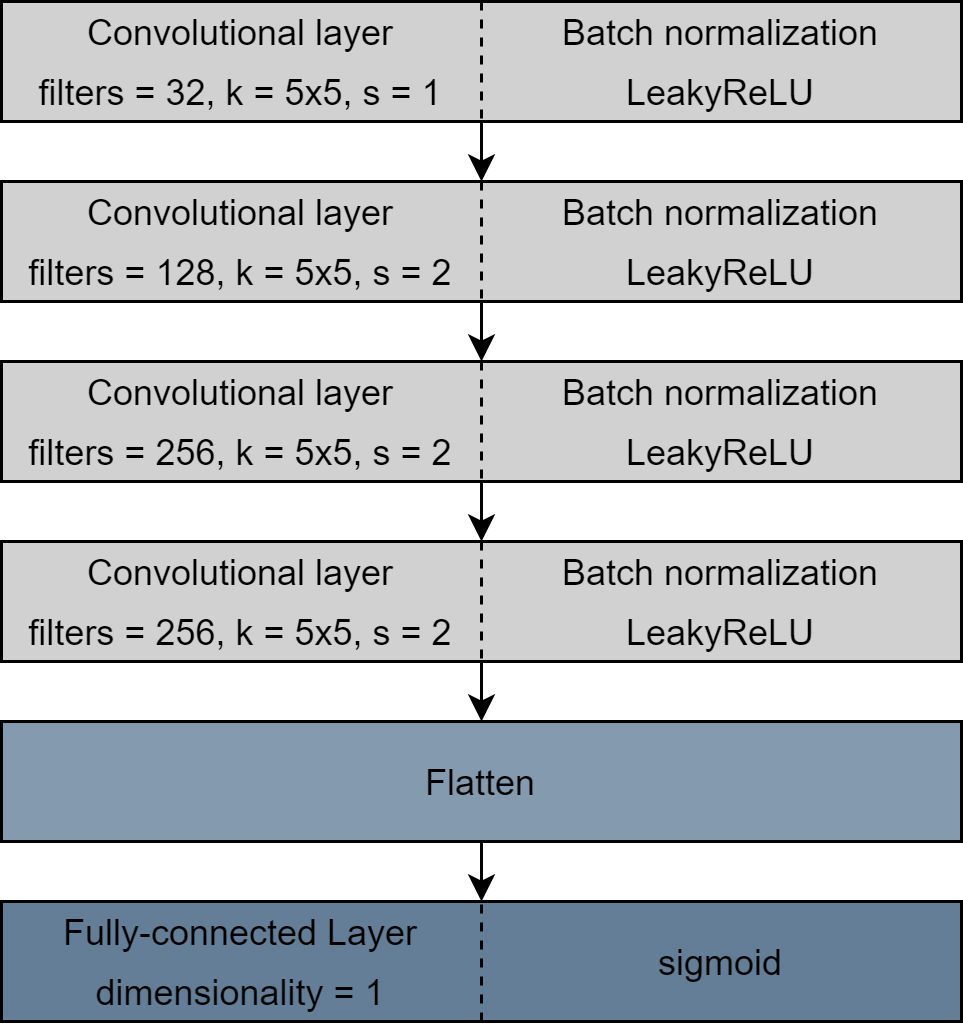
\includegraphics[width=10cm] {Models/vaegan_discriminator.png}
\centering
\caption{Discriminator architecture}
\label{fig:vaegan_dicriminator}
\end{figure}

\section{CycleGAN}

\begin{figure}[H]
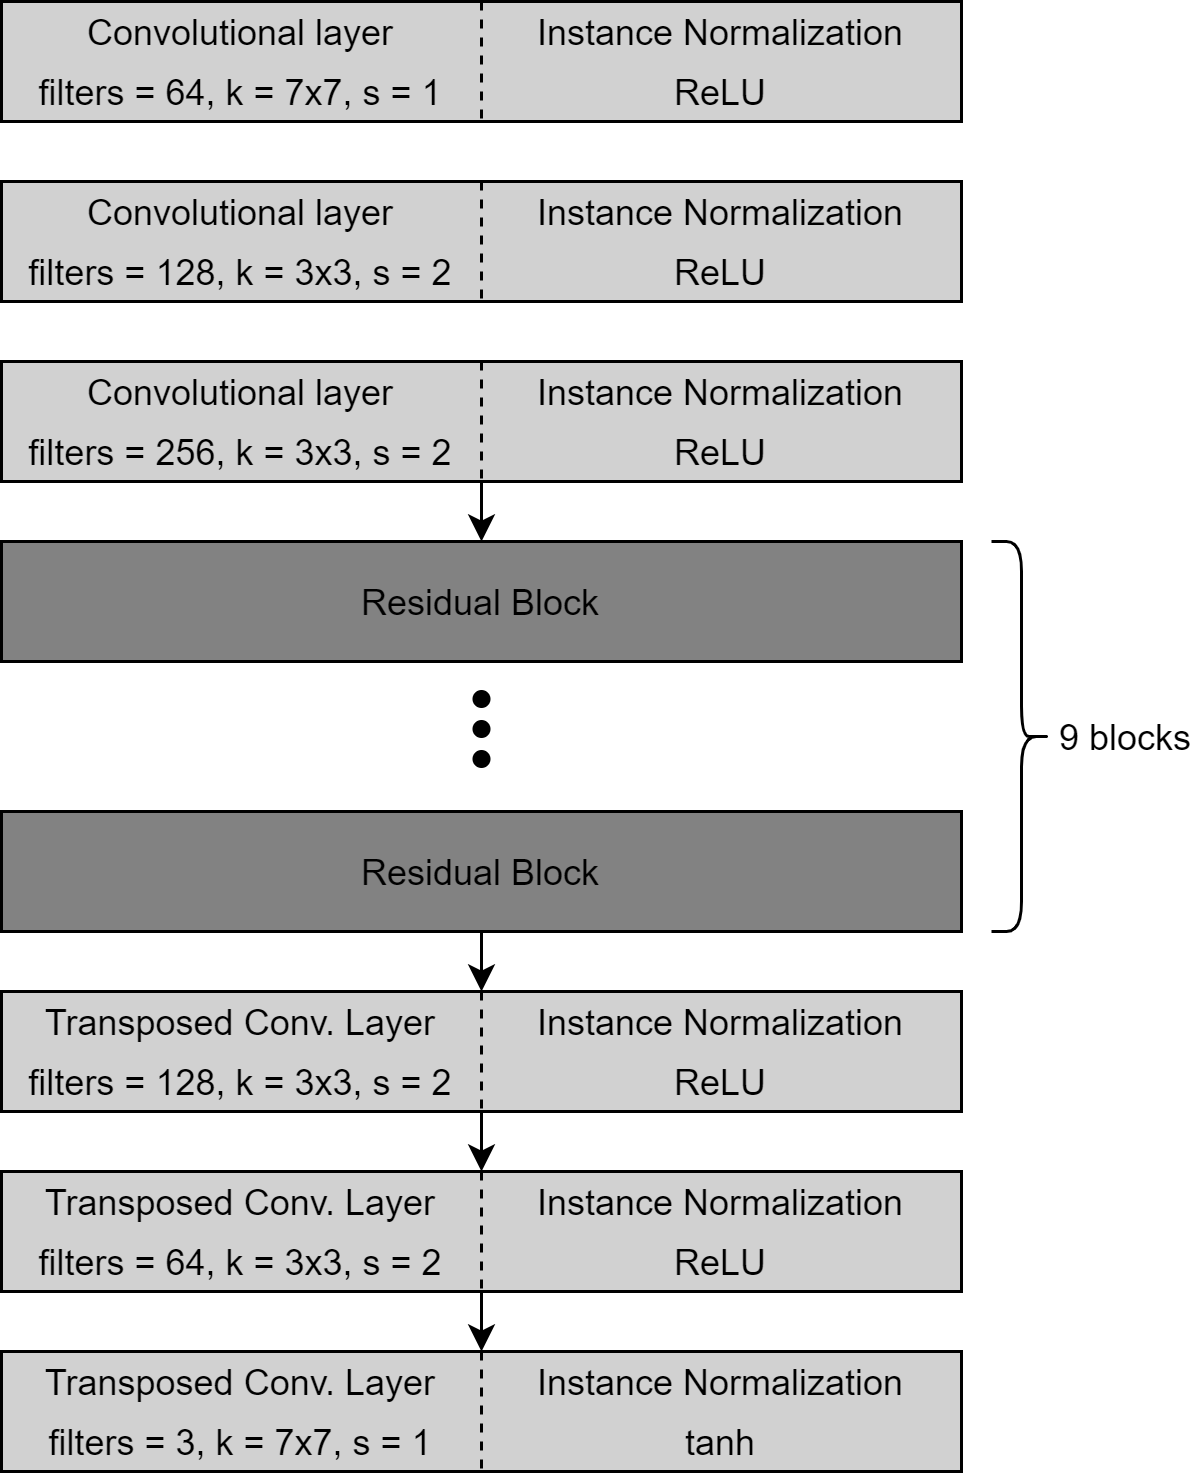
\includegraphics[width=13cm] {Models/cyclegan_generator.png}
\centering
\caption{Generator architecture}
\label{fig:cyclegan_generator}
\end{figure}

\begin{figure}[H]
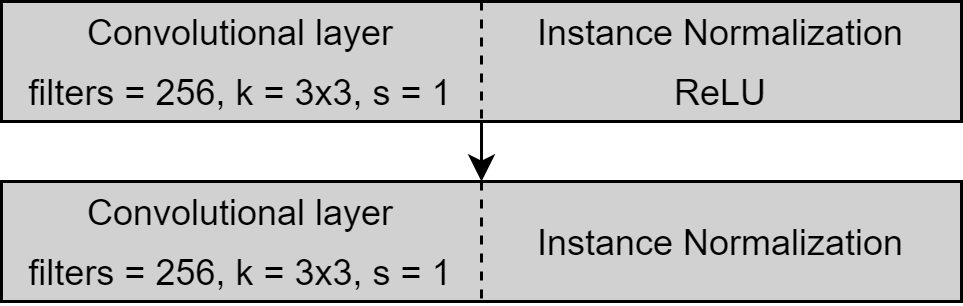
\includegraphics[width=10cm] {Models/cyclegan_residual.png}
\centering
\caption{Residual block architecture}
\label{fig:cyclegan_residual}
\end{figure}

\begin{figure}[H]
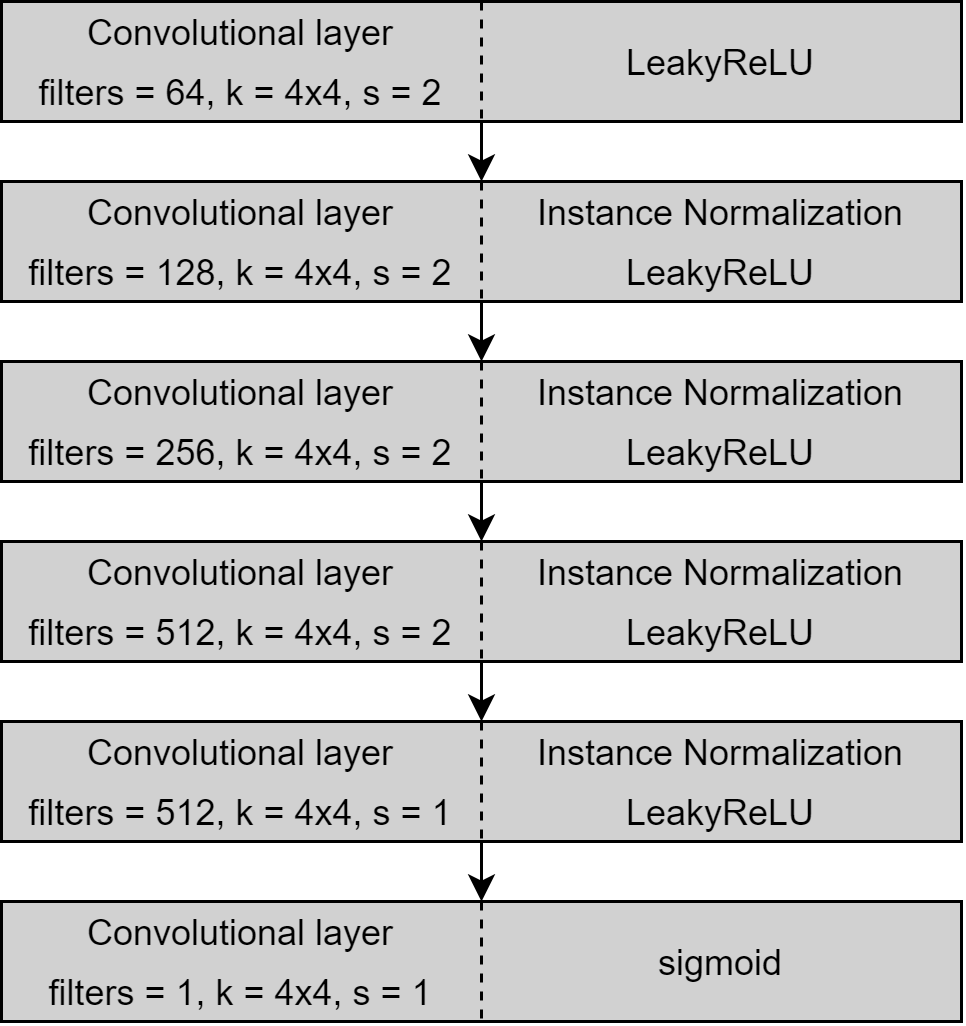
\includegraphics[width=10cm] {Models/cyclegan_discriminator.png}
\centering
\caption{Discriminator architecture}
\label{fig:cyclegan_generator}
\end{figure}